	\chapter{Einf\"uhrung in High-Performance-Computing} 
		\section{Amdahl's Law}
		Gegeben sei ein sequentielles Programm. Zerlegt man dieses in Teile, die theoretisch parallelisierbar sind, und jene, die in jedem Fall sequentiell laufen müssen, so ergibt sich die Gesamtlaufzeit $T$ als Summe 
		\begin{equation}\label{eq1:am}
		    T = t_p + t_s
        \end{equation}
        
        wobei $t_p$ die Laufzeit des parallelisierbaren Anteils und $t_s$ die des sequentiellen bezeichnet. Zu den unparallelisierbaren Anteilen zählen typischerweise Prozessinitialisierung oder Speicherverwaltung. Benutzt man ferner Hardware zum Ausführen des Programms, auf der insgesamt $n_P$ Prozessoren oder Prozessorkerne dauerhaft zur Verfügung stehen, so gilt für den sogenannten maximalen Speedup $S$:
		\begin{equation}
		    S = \frac{T}{t_s + \frac{t_p}{n_p}} \leq \frac{T}{t_s} = \frac{T}{T-t_p}
        \end{equation}	   
		
		Dabei wird das Verhältnis $\varepsilon = \frac{S}{n_P}$ auch als \gls{parallele Effizienz} bezeichnet. Als \Gls{Speedup} wird der Faktor bezeichnet, um den sich die Geschwindigkeit eines parallelen Programms gegenüber der sequentielle Vatiante verbessert. Abbildung \ref{1:am} zeigt diesen Speedup in Abhängigkeit von $n_p$ für verschiedene Verhältnisse von $\frac{t_p}{T}$.
		Allerdings hängt der sequentielle Anteil auch von der Parallelisierung selbst ab. Durch z.B. Prozessorkommunikation oder Synchronisation entsteht in der Gesamtlaufzeit ein zusätzlicher Summand	$t_{O(n_P)}$. In diesem Beispiel steigt der Anteil linear mit $n_P$. Dies ist jedoch nicht zwingend der Fall. Damit ergibt sich der maximale \Gls{Speedup}:		
		\begin{equation}
		    S = \frac{T}{t_s + t_{O(n_P)} + \frac{t_p}{n_p}} \leq \frac{T}{t_s} = \frac{T}{T-t_p}		
		\end{equation}
		
		Diese Kurve konvergiert nun nicht mehr gegen $\frac{T}{t_s}$, sondern erreicht ein Maximum, um danach wieder abzufallen (Abb. \ref{1:am_prax}). In der Praxis ergibt sich ein Optimum, eine Anzahl von Prozessoren, bei der sich der maximale \Gls{Speedup} erzielen lässt. Eine Vergrößerung dieser Anzahl hat einen negativen Effekt, da der Geschwindigkeitsgewinn durch die weiteren Prozessoren den Aufwand der Prozessorkommunikation nicht mehr kompensiert.


		\section{Gustafson's Law}
		Amdahl stellte mit seinem Gesetz eine worst-case Abschätzung auf, bei der sich die Laufzeit mit der Zahl der Prozessoren linear verbessern lässt. Amdahl geht dabei von einer festen Problemgröße aus. Gustafsons Gesetz hingegen geht von einem festen Zeitfenster aus. In diesem wächst die Problemgröße mit Anzahl der Prozessoren. Mit dieser Zahl wächst linear auch die Größe der Aufgabe, die unter den Voraussetzungen gelöst werden kann.

		Setzt man $P=t_p/T$ lässt sich \ref{eq1:am} umschreiben:
		\begin{equation}
			1 = (1 - P) + P
		\end{equation}

    	Lässt sich der parallele Anteil unter Vernachlässigung von $t_{O(n_P)}$ gleichzeitig auf $n_P$ Prozessoren ausführen, so gilt für den \Gls{Speedup}:
    	\begin{equation}
        	S(n_P) = (1 - P) + n_P P
    	\end{equation}
		
		Der parallele Anteil wächst also linear mit der Anzahl der Prozessoren. Im Gegensatz zu Amdahl wird der sequentielle Anteil mit zunehmenden $n_p$ bedutungslos, wirkt also nicht beschränkend.
		 
        \section{Amdahl vs. Gustafson}		
        Nach Amdahl ist die \gls{parallele Effizienz}:
        \begin{equation}
            \varepsilon_{\text{Amdahl}}(n_P)    = \frac1{n_P}\cdot \frac1{(1-P)+P/n_P} = \frac1{n_P(1-P)+P}
        \end{equation} 
        Nach Gustafson ist die \gls{parallele Effizienz}:
        \begin{equation}
			\varepsilon_{\text{Gustafson}}(n_P) = 1 - \frac{n_P-1}{n_P}\cdot (1-P) = P +\frac{1-P}{n_P}
        \end{equation}
		Laut Amdahl geht die \gls{parallele Effizienz} im Limit einer großen Prozessorzahl immer gegen null, bei Gustafson existiert eine untere Schranke $P$:
        \begin{gather*}
        	\lim\limits_{n_P \rightarrow \infty}\varepsilon_{\text{Amdahl}}(n_P)    = 0 \\        
        	\lim\limits_{n_P \rightarrow \infty}\varepsilon_{\text{Gustafson}}(n_P) = P
        \end{gather*}
        
        Welches Modell nun Anwendung finden sollte, hängt von der Problemstellung ab. Gustafsons Gesetz sollte auf Probleme angewandt werden, falls sich die Promblemgrö\ss e auf die Parallelisierung anpassen lässt, andernfalls Amdahl. In jedem Fall geben Amdahl und Gustafson eine Ober- und Untergrenze für den \Gls{Speedup} an. 
        
        \begin{figure}[h]
			\centering
    		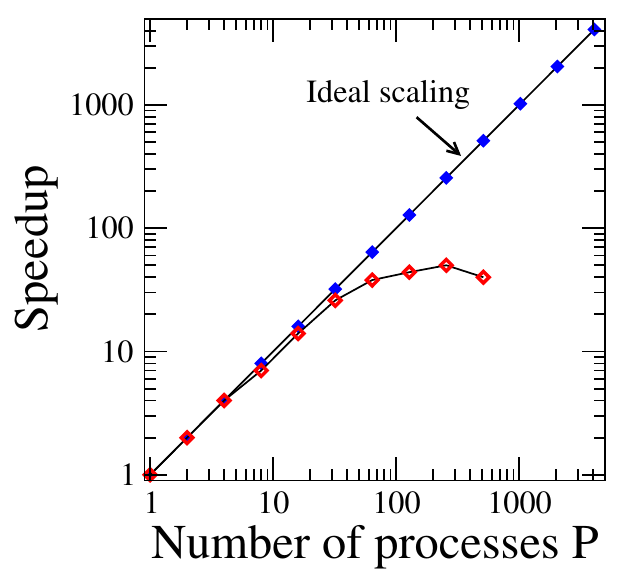
\includegraphics[height=0.4\textwidth]{/home/kat10110/script/chapter1/pictures/Amdahl_praxis.png}
    		\caption[Speedup laut Amdahl mit Prozesskommunikation]{Der Speedup laut Amdahl bei einer bestimmten Zahl an Prozessoren unter Berücksichtigung von Prozessorkommunikation. Ab einer bestimmten Anzahl nimmt der Speedup wieder ab. (doppelt-logarithmische Skala) \autocite{carch}}
    		\label{1:am_prax}
		\end{figure}
        
        \newpage
		\begin{figure}[h]
			\centering
    		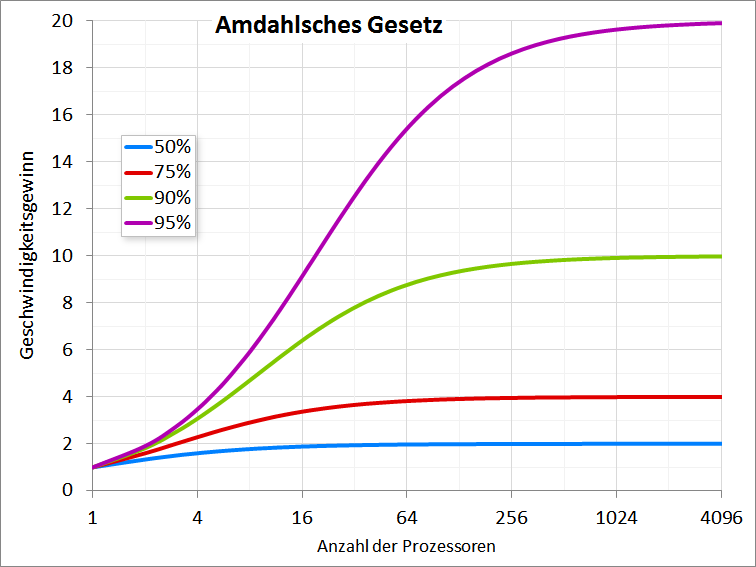
\includegraphics[height=0.5\textwidth]{/home/kat10110/script/chapter1/pictures/Amdahl.png}
    		\caption[Speedup laut Amdahl ohne Prozesskommunikation]{Der Speedup laut Amdahl bei einer bestimmten Zahl an Prozessoren ohne Berücksichtigung von Prozesskommunikation für verschiedene Verhältnisse von $t_s/T$. Der Speedup konvergiert schnell gegen $T/t_s$. (einfach-logarithmische Skala) \autocite{wikiAmdahl}}
    		\label{1:am}
		\end{figure}
		
		\newpage
		\section{Roofline Model}
		\begin{figure}[t]
			\centering
	    	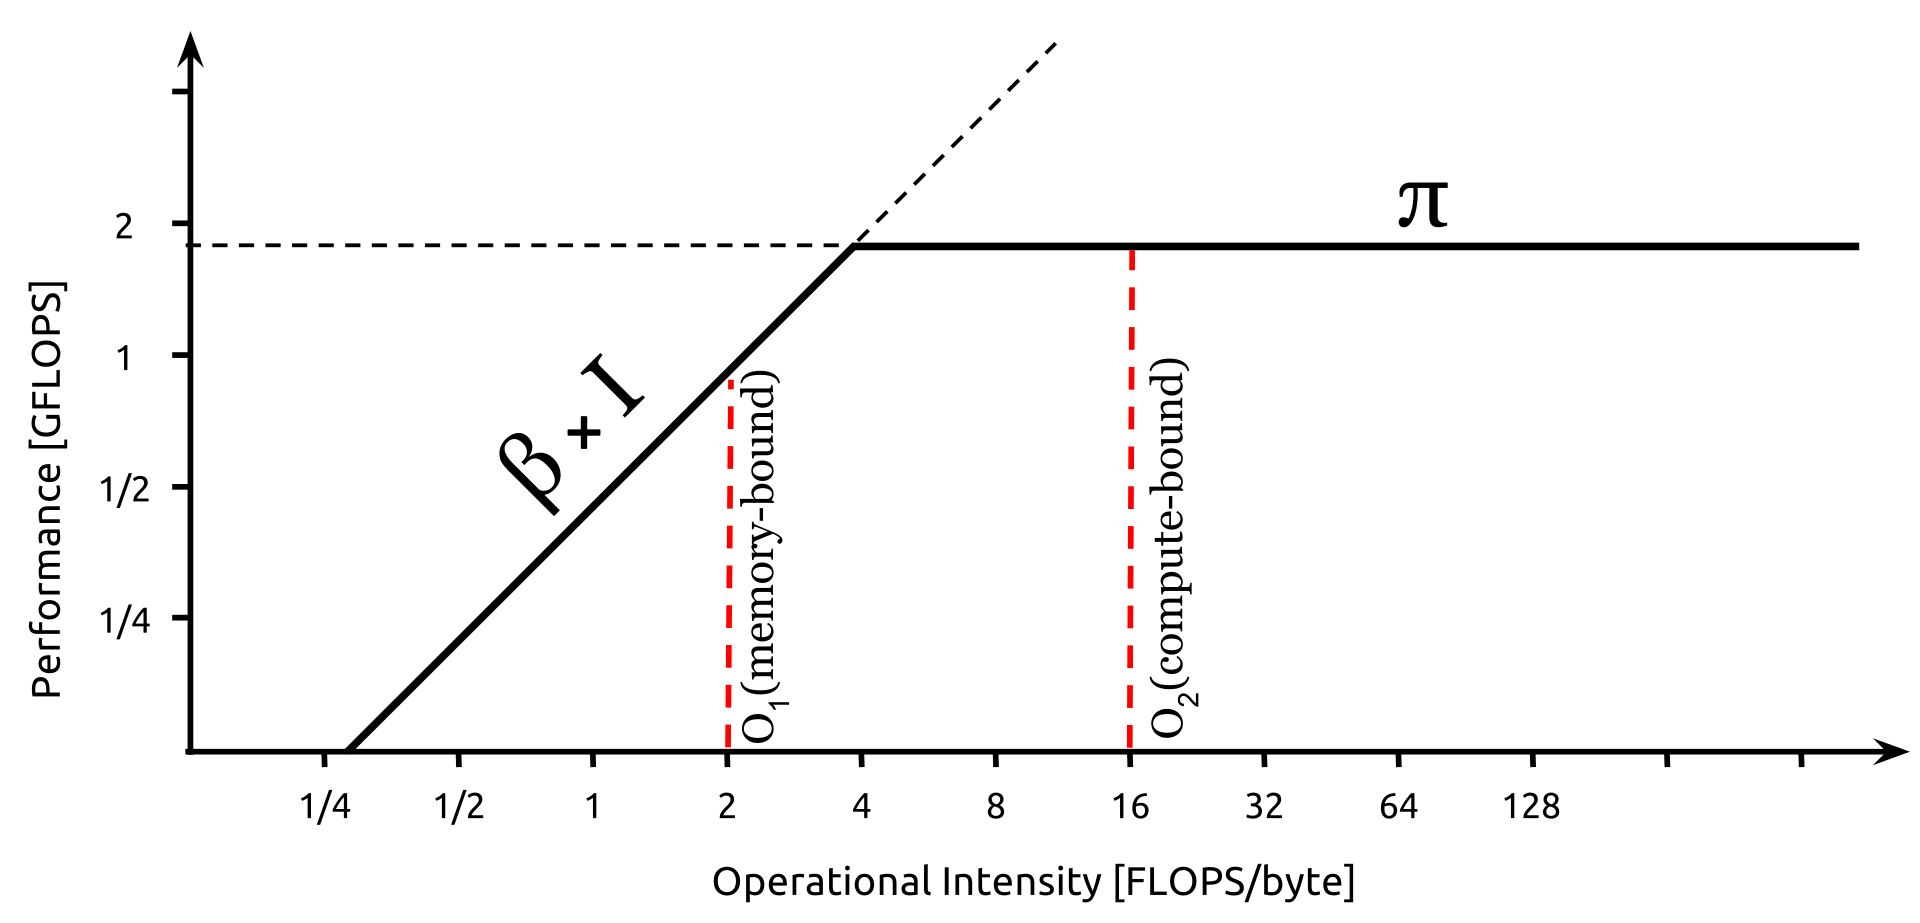
\includegraphics[height=0.4\textwidth]{/home/kat10110/script/chapter1/pictures/roofline_model_0.png}
    		\caption[Roofline Modell - naiv]{Die Performance $P$ als Funktion der arithmetischen Intensität $I$ bei doppelt-logarithmischer Skalierung. (naives Modell) \autocite{wikiRLM}}
    		\label{1:rl0}
		\end{figure}

		\begin{figure}[t]
			\centering
	    	
\includegraphics[height=0.4\textheight]{/home/kat10110/script/chapter1/pictures/roofline_model_1.png}
    		\caption[Roofline Modell - \textit{bandwidth ceiling}]{Die Performance $P$ als Funktion der arithmetischen Intensität $I$ bei doppelt-logarithmischer Skalierung. Es existiert ein negativer Offset aufgrund von \textit{bandwidth ceiling}. Dieses Verhalten entsteht durch fehlende Speicheroptimierung. \autocite{wikiRLM}}
    		\label{1:rl1}
		\end{figure}
	
		\begin{figure}[t]
			\centering
	    	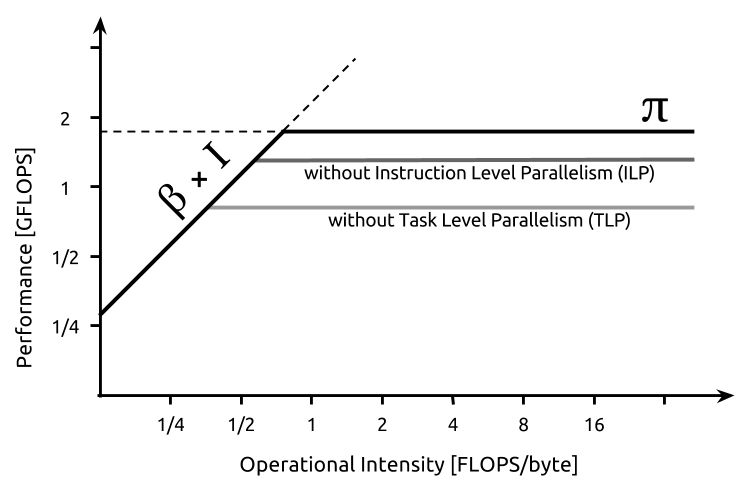
\includegraphics[height=0.35\textheight]{/home/kat10110/script/chapter1/pictures/roofline_model_2.png}
    		\caption[Roofline Modell - \textit{in-core ceiling}]{Die Performance $P$ als Funktion der arithmetischen Intensität $I$ bei doppelt-logarithmischer Skalierung. Es existiert ein e Beschränkung der \textit{peak performance} aufgrund von \textit{in-core ceiling}. \autocite{wikiRLM}}
    		\label{1:rl2}
		\end{figure}

		\begin{figure}[b]
			\centering
    		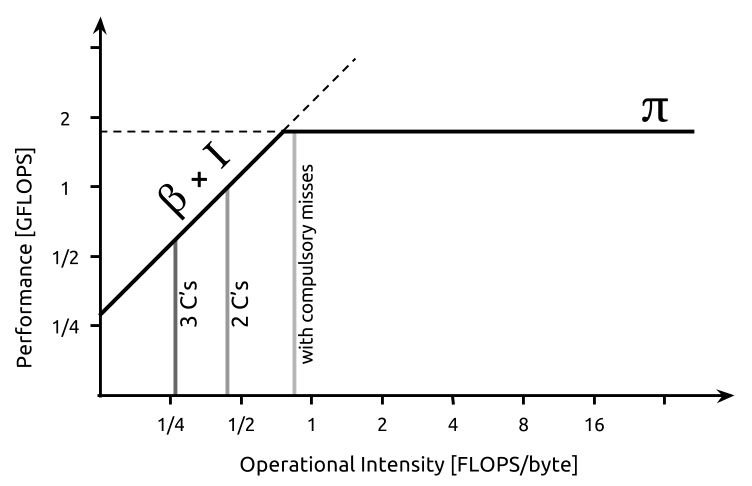
\includegraphics[height=0.35\textheight]{/home/kat10110/script/chapter1/pictures/roofline_model_3.png}
	    	\caption[Roofline Modell - \textit{locality walls}]{Die Performance $P$ als Funktion der arithmetischen Intensität $I$ bei doppelt-logarithmischer Skalierung. $I$ lässt sich aufgrund der Cachetopologie über bestimmte \textit{locality walls} hinaus nicht steigern. rechts: \textit{compulsory misses}, C3: zusätzlich \textit{capacity-} und \textit{conflict misses}, C2: zwei von drei \autocite{wikiRLM}}
    		\label{1:rl3}
		\end{figure}
		
		Sei eine \Gls{Arbeit} $W$ gegeben, die ein Programm oder auch nur eine bestimmte Funktion verrichten muss. $W$ wird üblicherweise angegeben in einer Zahl an Fließpunktoperationen (engl. floating point operations, FLOPs). Abhängig von der Problemstellung kann aber auch ein anderes Maß gewählt werden. $W$ ist eine Eigenschaft des Programms und hängt daher nur unwesentlich von der Hardware ab.
		
		Der \Gls{Datenverkehr} $Q$ (engl. memory traffic) bezeichnet die Zahl an Bytes, die während des Ausführens des Programms insgesamt transferriert wird. $Q$ ist im Wesentlichen eine Eigenschaft der Hardware und hängt z.B. von der Cachehierarchie ab.

		$I = W/Q$ bezeichnet die \gls{arithmetische Intensität}. Dabei handelt es sich um die Anzahl an Operationen pro transferriertes Byte. Die Einheit ist FLOPs/Byte.
		Das sogenannte naive Roofline Modell geht von nur zwei Parametern aus, der \textit{\Gls{Peak Bandwidth}} $\beta$ und der \textit{\Gls{Peak Performance}} $\pi$. Lediglich $I$ ist variabel. Die \textit{\Gls{Peak Performance}} ist eine feste Hardwaregröße, die vom ausführenden Gerät abhängt. Diese Größe lässt sich aus den entsprechenden Datenblättern ablesen. Die \textit{\Gls{Peak Bandwidth}} wird normalerweise durch \textit{benchmarking} bestimmt (später mehr). Die erreichbare \Gls{Performance} kann dann wie folgt berechnet werden:
		
		\begin{equation}
			P = \min \left\{ \begin{array}{ll} \pi \\
			\beta\times I \\ \end{array}\right.
		\end{equation}
		Abbildung \ref{1:rl0} zeigt dieses Verhalten exemplarisch. Der Schnittpunkt der beiden Linien $I^{\prime} = \pi/\beta$ wird als \textit{ridge point} bezeichnet und charakterisiert die eingesetzte Hardware entscheidend. Er bezeichnet jenes $I$, das ein Programm mindestens erreichen muss, um bei gegebener Hardware diese maximal auszureizen. Gleichzeitig beschreibt er den Punkt, ab der eine Erhöhung von $I$ keinen Effekt mehr hat. Bei Programmen, für die $I < I^{\prime}$ gilt, spricht man von \textit{memory bound}, andernfalls von \textit{compute bound}.
		
		Beim naiven Modell handelte es sich um eine best-case Abschätzung. In der Praxis gibt es allerdings weitere Limitierungen. Die Abbildungen \ref{1:rl1}, \ref{1:rl2} und \ref{1:rl3} zeigen folgende Fälle:
		
		\begin{enumerate}		
		\item Kommunikation: bandwidth ceilings
		\item Berechnung: in-core ceilings
		\item Lokalität: locality walls
		\end{enumerate}	